\section{Simulation Techniques and Physics Scenarios\label{simSetup}}


\begin{figure}%[!htb]
\begin{center}
\includegraphics[scale=0.6]{figures/LHCring.pdf}
\end{center}
\vspace{-0.6cm}
 \caption{Schematic view of the LHC its 8 insertion regions (IRs) and circulating beam directions.
  \label{LHCring}}
\end{figure}

We study three sources of background as mentioned earlier mainly for IR1 but we also investigate cleaning leakage to IR5 in various scenarios. Near-by or local beam-gas considers contributions up to 547~m deep in the arc. This has been the largest source of machine-induced background to the experiments in Run~I in 2011~\cite{nimPaperRod} and 2012~\cite{atlasBKGPaper2012}. The other two sources, betatron halo and off-momentum halo induced particle showers, are due to leakage from the IR7 and IR3 cleaning insertions, respectively. This means B1 and B2 have quite a different impact on IR1 and IR5 when following the beam directions as shown in Fig.~\ref{LHCring}.

The simulation of background in the LHC can be very demanding in terms of CPU. Detailed shower simulations are required along several hundred meters, or many millions of primaries have to be tracked to get sufficient particles leaking to collimators in IR1 or IR5 -- which by design are many orders of magnitudes lower than protons hitting the primary collimators. Two Monte-Carlo simulation codes were used as main tools: SixTrack with collimation~\cite{SixTrackRef} for particle tracking and \fluka~\cite{flukaRef1,flukaRef2}~for particle showering.

The IR1 layout of the present machine is shown in Fig.~\ref{nominalLHC_layout} with the IP1 at s~=~0. By design, the left and the right side are symmetric for incoming beams. Also the layout of the outgoing side is symmetric for both beams. For our purposes, shower evaluation from different background sources, it is sufficient to use only half of the layout for the incoming beam in IR1. The right side of IP1 is used for both beams. For illustration, the \fluka~geometry of the machine-detector interface region is shown in Fig.~\ref{flukaGeo_nominal}.



\subsection{Betatron Halo simulations}
The simulation is performed in two main steps: First, we use SixTrack for particle tracking in order to obtain the leakage onto the TCTs in the IRs, using the same method as described in Ref.~\ref{nimPaperRod}. To be CPU efficient, only a halo proton distribution is tracked not the full beam with its core that is usually many orders of magnitude more dense. Tracking is performed through a magnetic field lattice, usually prepared using MadX~\cite{madx}, and the LHC collimatiors of which only the jaws are modeled. We also assume a perfect machine, neglecting any uneven jaw surfaces or edges\footnote{Previous studies~\cite{roderikSimMeasPaper} have shown that, if one includes machine errors, the leakage on to the TCTs could differ by a factor of about 2 to 3.}.

The beam halo is usually simulated in horizontal (h) and vertical (v) distributions. These are flat in one plane and Gaussian in the other (for more information see also~\cite{chiarasThesis}). When a collimator is hit, a built-in, recently updated Monte-Carlo model~\cite{claudiasThesis} decides on the physics process. Protons continue in the lattice until they dissociate in an inelastic interaction with the collimator material or (in a post-processing step) are lost on the aperture. As a result, loss locations around the ring can be identified and protons absorbed by the TCTs serve in second step as starting conditions in \fluka. Particle interaction and transport are calculated in \fluka~in a user-defined geometry. The geometry was built up to 547~m of the right side of IR1 for the present LHC machine, for HL-LHC scenarios the geometry (\fluka~model from 2013--14) reaches up the tertiary collimators of around 215~m including the long straight section of IR1 (LSS1).

When halo protons interact with the jaw material of the TCTH or TCTV shower particles are created and stream towards the experiment. We apply a electron, photon production and hadron, muon, neutrino transportation cut of 20~MeV. Information of every particle which makes it to an imaginary (x,y)-plane at 22.6~m away from the IP, essentially between the triplet magnets and the TAS, is recorded and written out and provided to the experiments as input to further studies of the detector response. The left plot of Fig.~\ref{tctHits} shows part of the \fluka~geometry and in green the simulated locations of inelastic interactions in an horizontal collimator TCTH.4L1 with absorbed protons from an horizontal and vertical halo distribution. On the right of Fig.~\ref{tctHits} one can see how deep these positions are with respect to the jaw surface shown for the collimator pair of IR1. This depth distribution is shown here as an example, but we can note that the shallower the distribution is, the more of the created shower is not confined and contributes to background at the interface plane.

\subsubsection{Rate normalisation}



We normalised the distributions at the interface plane by the initial proton intensity that was present in the machine for a given scenario and by the IR7 TCP-to-TCT conversion factor which is throughout this report the number of halo protons on IR7 TCPs (sum of TCP.D6, TCP.C6 and TCP.B6 for a horizontally, vertically aligned and skew collimator). Taking the sum of absorbed protons of all TCPs is closer to the measurement technique where losses are usually normalised to the peak loss measured with the beam loss monitor\footnote{There are more than 3000 BLMs installed in the LHC, their primary purpose is to provide a beam abort in case of need.} that is attached to the collimator. Assuming equal loss rates on the horizontal and vertial TCP, we give equal weights to horizontal and vertical halo simulations and losses per simulation case are summed and then averaged. Initial particles that can be lost are the number of bunches, $N_{\mathrm{bunch}}$, times the bunch intensity, $I_{\mathrm{bunch}}$. To estimate a loss rate, we include also a time $\tau_\mathrm{stable \, beam}$ to indicate stable beam operation assuming 100 hours of beam life time. This means that in linear approximation, the whole beam intensity would be lost over the time $\tau_{\mathrm{stable \, beam}}$ on the collimators. Luminosity losses are not included in this lifetime. Throughout this report the normalisation of halo shower results was done using Eq.~\ref{eqNormHalo} with $h$ and $v$ representing the horizontal and vertical halo simulations. Inside the square brackets, $N$ is the number of absorbed protons and the subscripts indicate the collimator. The content of the square brackets, the leakage numbers, are listed in App.~\ref{leakageFactorsIR7}, for various simulation cases.

\begin{equation} \label{eqNormHalo}
R = \frac{N_{\mathrm{bunch}} \cdot I_{\mathrm{bunch}}}{\tau_{\mathrm{stable \, beam}}} \times \Bigg[ \frac{1}{2} \cdot \Big( \frac{N_{\mathrm{TCTV}} + N_{\mathrm{TCTH}}}{N_{\mathrm{TCP.IR7}}}\Big)_{\mathrm{h}} + \Big( \frac{N_{\mathrm{TCTV}} + N_{\mathrm{TCTH}}}{N_{\mathrm{TCP.IR7}}} \Big)_{\mathrm{v}}  \Bigg]
\end{equation}


\begin{figure}%[!htb]
\begin{center}
\includegraphics[width=0.9\textwidth]{figures/IR1_layout_runII.pdf}
\end{center}
\vspace{-0.6cm}
 \caption{Machine layout for the nominal LHC (as in Run I and II) of IR1 with IP1 at s~=~0 and incoming beam from the left. Highlighted are the tertiary collimators (TCT4) at around -147~m. TCLs are debris collimators for the outgoing beam.
  \label{nominalLHC_layout}}
\end{figure}


%% \begin{figure}
%% \begin{center}
%% 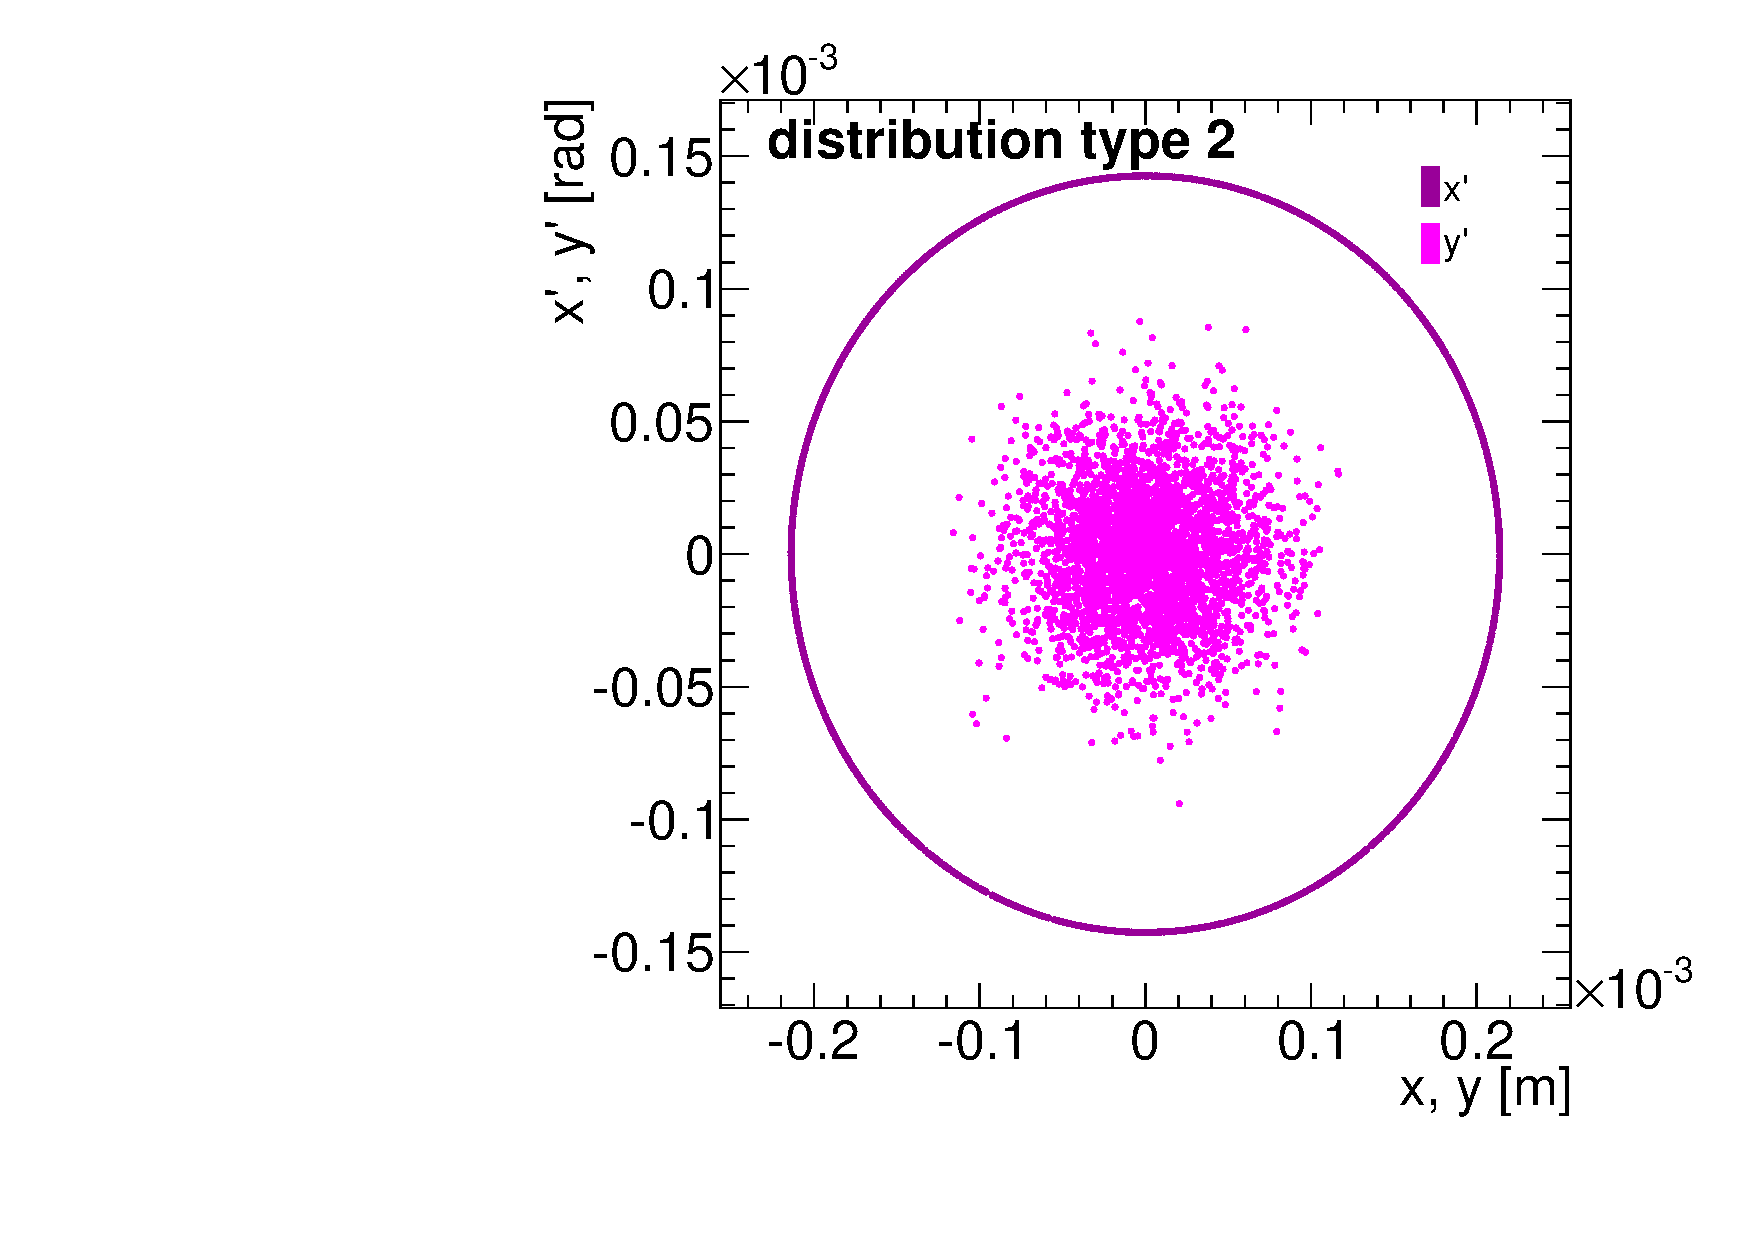
\includegraphics[width=0.48\textwidth]{figures/phasespace_d2}
%% 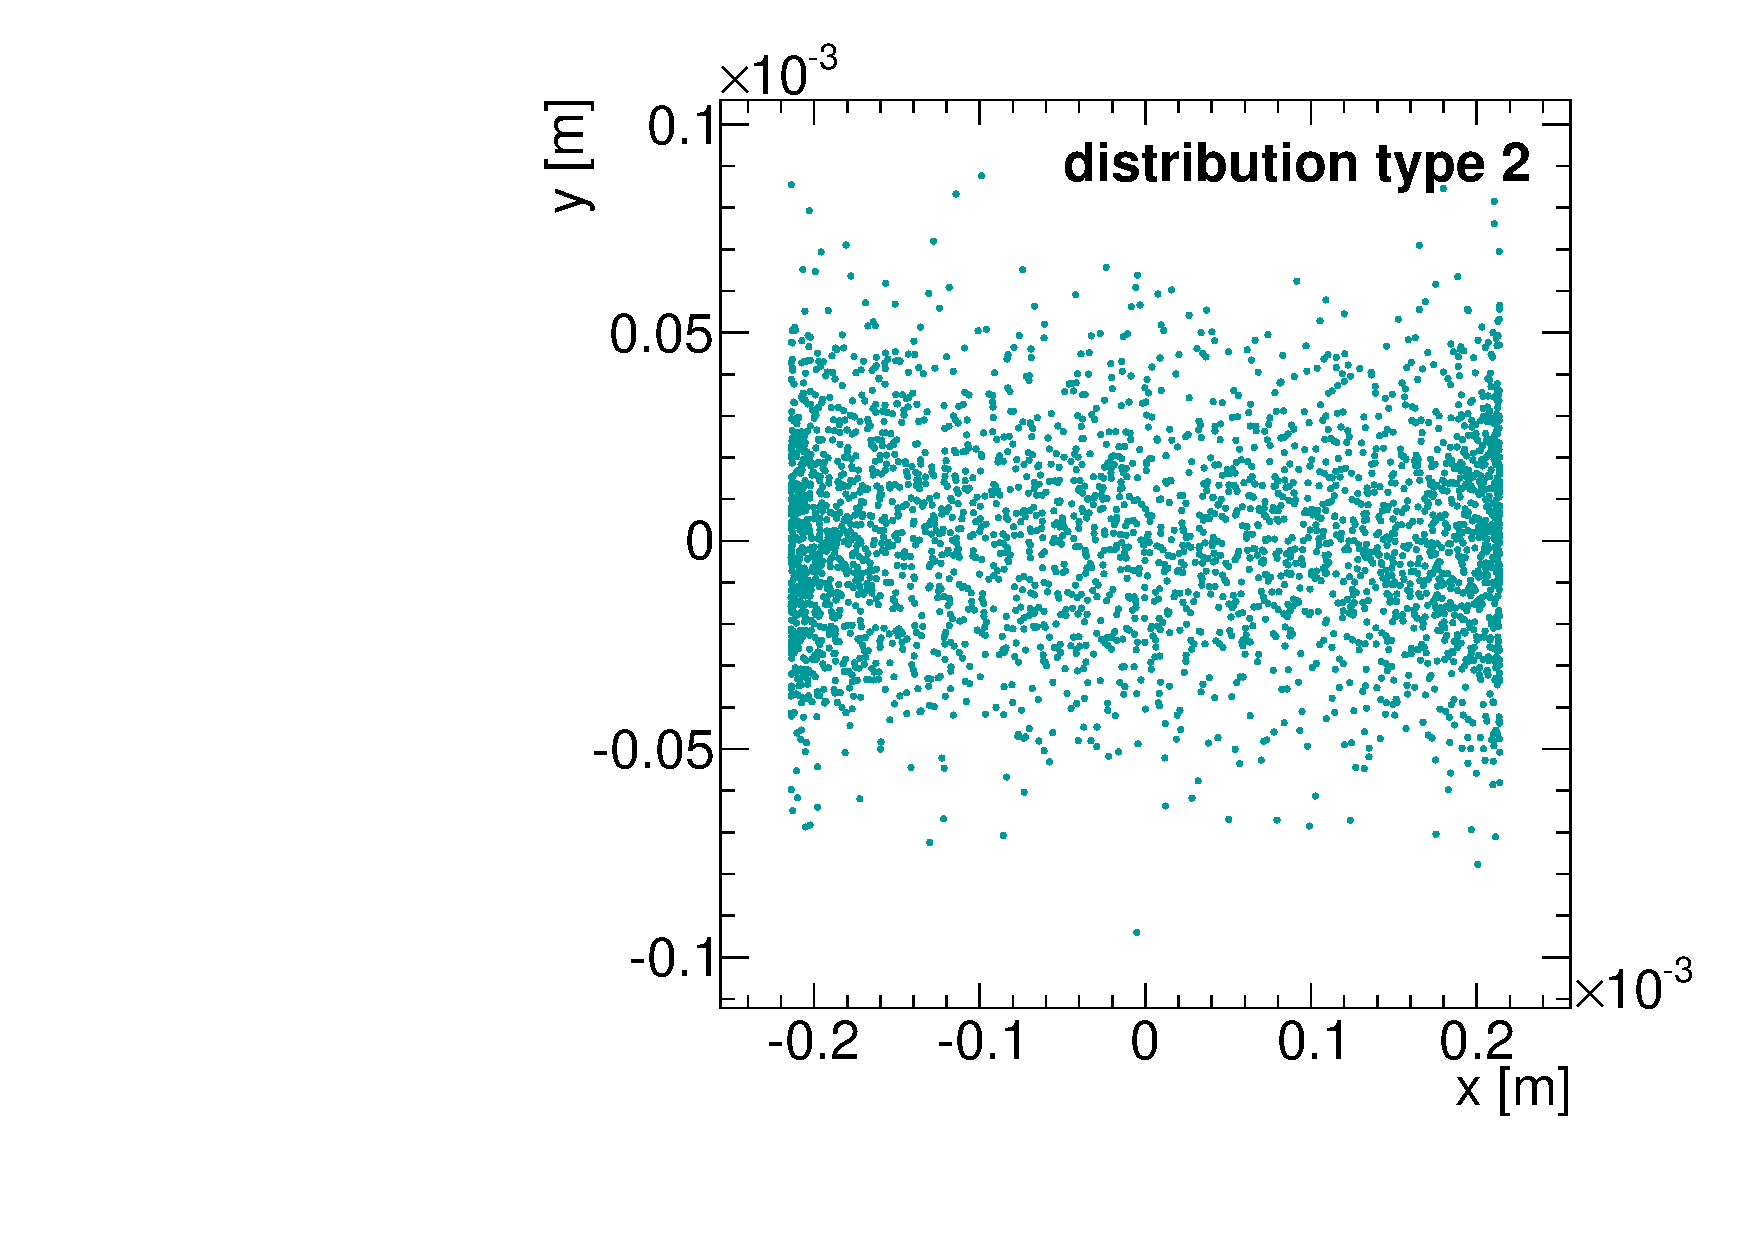
\includegraphics[width=0.48\textwidth]{figures/realspace_d2}
%% \end{center}
%% \caption{Initial halo distribution of type 2 in phase-space (left) and real space (right) is generally used in horizontal halo simulations with SixTrack.
%% \label{haloExamples}}
%% \end{figure}


\begin{figure}%[!htb]
\begin{center}
\includegraphics[width=0.9\textwidth]{figures/IR1_interfaceplane.pdf}
\end{center}
\vspace{-0.6cm}
 \caption{Example of the interface region in \fluka: x-z cut of \fluka~geometry zoomed into the interface region between detector and machine. A virtual plane at z~=~22.6 m (interface plane) is used as location, where information of particles entering the detector region are recorded. Each color defines a different material, e.g.~light grey is concrete. The tunnel part is the same for LHC and HL-LHC, only beamline elements are different.
  \label{flukaGeo_nominal}}
\end{figure}


\begin{figure}%[!htb]
\begin{center}
  \includegraphics[width=0.4\textwidth]{figures/6500GeV/xz_6500GeV_b1_TCT4.pdf}
  \includegraphics[width=0.4\textwidth]{figures/6500GeV/inelposition_sum_HALOB1.pdf}
\end{center}
\vspace{-0.6cm}
 \caption{Left: View at the (x,z)-plane of points of inelastic interactions in TCTH from an Run~II halo simulation case zoomed into inner collimator parts. They were obtained by SixTrack and transformed to the positions of the TCT in the \fluka~coordinates. Right: The same positions measured from the jaw surface in the TCTH.4 and those in the TCTVA.4 are shown.
  \label{tctHits}}
\end{figure}


\subsection{Beam-Gas simulations \label{BGdescript}}

We simulate local beam-gas interactions in a \fluka~geometry up to $s$ = 546.6~m of IR1. Inelastic proton-gas interactions are sampled all along $s$ and these positions used to be only on the ideal orbit of the beam trajectory. We introduce a new way of sampling taking into account the transverse extension of the beam which is described in detail further below.
Like for the beam-halo simulations, information of each shower particle with energy above 20~MeV and reaching the virtual interface plane at 22.6~m is recorded.

If one has a non-flat pressure profile of different residual molecule species, one can either reweight the uniformly sampled proton-gas interactions at run-time or in a subsequent step, if one keeps the information of the initial s-position of the interacting proton of each particle at the interface plane. We have used the first method in the beam-gas simulations in an HL-LHC scenario described in Ref.~\cite{kweeIpac14}. The second method, reweighting the distributions at the interface plane in a sub-sequent step, is used for beam-gas in Run~I (2012) and Run~II (2015). For the simulation cases shown here, nitrogen was chosen as collision partner as approximation of the real gas species which has its atomic number in between carbon and oxygen. Also, the simulation of the real pressures are calibrated against nitrogen and given in nitrogen equivalent. Most dominant gas species are H$_2$, CH$_4$, CO and CO$_2$.

\begin{table}
   \centering
   \caption{Inelastic atomic cross-sections for a specific atom at rest with an LHC beam proton. Extracted from \fluka.}
   \begin{tabular}{c|c|c}\hline
     &  $\sigma$ [mb] &  $\sigma$ [mb] \\
       & E$_{beam}$ = 4 TeV   & E$_{beam} =$ 6.5 TeV \\ \hline\hline
       H & 37.1 & 38.4 \\
       C & 260& 269 \\
       O & 318 & 329 \\
       \hline
   \end{tabular}
   \label{tab:atomicXsections}
\end{table}

The inelastic cross-sections are listed in Tab.~\ref{tab:atomicXsections} and were extracted from \fluka. The cross-sections were indicated as an interaction probability per unit length per atom (macroscopic cross-section), e.g.~[$\sigma^{\textrm{macro}}$] = $\frac{1}{cm}$. To convert to the microscopic cross-section, one has to divide by the number of atoms per unit volume, eg.~atoms/cm$^3$.

These were used to compute rate of the interaction probability of a specific gas $i$ per beam proton, time and unit lenght which is the product of the number of available gas molecules (or atoms), given by the density $\rho_i$ of that species, and its cross-section $\sigma_i$ divided by the revolution period of the beam $T_{\mathrm{rev}}$:
\begin{equation} \label{eq2}
p_{\mathrm{int},i} = \sigma_{i} \cdot \rho_{i}(s) \cdot \frac{1}{T_{\mathrm{rev}}}
\end{equation}

The method to reweight the particle distribution at the interface plane, simulated with a uniform pressure profile, to any given real profile, is the same as in Ref.~\cite{nimPaperRod}. We write down the weights to be applied to each bin $j$ that is already in a binning-independent representation (division by bin width or bin area) and already normalised by the number of simulated beam-gas interactions. The weight is thus the interaction rate in bin $j$:

\begin{equation} \label{eq3}
\mathrm{weight}_j = N_{\mathrm{protons}} \cdot p_{\mathrm{int}}^{\mathrm{tot}} (s_j) \cdot \Delta s_{j} 
\end{equation}

with the total rate of interaction probabilities of each atom $i$ at the position $s_j$ 
\begin{equation*} 
  p_{\mathrm{int}}^{\mathrm{tot}} (s_j) = \Sigma_i \, p_{\textrm{int},i}
\end{equation*}

and the length $\Delta s_{j}$ over which the interaction probability is valid.

\subsection{New simulation techniques}
Previous studies as in Ref.~\cite{nimPaperRod} used methods relying on approximations of either of the beam or its trajectory. One approximation is that the transverse beam size was neglected. In particular, at the entrance of the triplet the beamsize is very large, see as example beam sizes in Fig.~\ref{twissfileBS}, and beam-gas interactions do not only occur on the central trajectory, which maybe influence the distribution at the interface plane. Another improvement in the simulations is the inclusion of the crossing angle which was present in the real machine configuration right from start-up of the LHC.

\subsubsection{Setup to include the beam size}

In order to account for the beam size, an input file with coordinates of inelastic beam-gas events was created by dumping in \fluka~positions of the trajectory with different starting positions. The ideal orbit goes through (0,0) in (x,y) at the IP. Assuming a gaussian distribution of the beam particles one can produce matched phase space coordinates in the transverse plane, as shown in Fig.~\ref{ip1_gauss}, at the IP where the optical functions are $\alpha=0$, $\beta=\beta^*$. Using a normalised coordinate system, the phase space coordinates were calculated as in Eq.~\ref{eq1}

\begin{equation} \label{eq1}
  \begin{split}
x = & \, \sqrt{\beta \epsilon_{geo}} \cdot X \\
x' = & \sqrt{\frac{\epsilon_{geo}}{\beta}} \, \big( X' - \alpha X \big)
  \end{split}
\end{equation}

with $\epsilon$ being the geometric emittance, $\alpha, \beta$ and $\gamma$ the usual twiss parameters from the definition of the emittance in $\epsilon_{geo} = \gamma x^2 + \beta x'^2 + 2 \alpha x x'$. $(X,X')$ are the normalised phase space coordinates, used for the sampling, while $(x,x')$ are the physical phase space coordinates, used in the simulations as initial conditions in \fluka~to create the trajectory. 1000 trajectories were created and randomly 10 transverse positions per longitudinal coordinate were chosen. To illustrate the final input file to \fluka~e.g.for the 2015 Run~II case, see beam-gas sampling positions in Fig.~\ref{BGASflukaInp}. The Run~I case is very similar (not shown). As example we visualise the beam sizes for the Run~II case in Fig.~\ref{twissfileBS} and within the triplet as calculated based on $\beta-$functions\footnote{given by $\sigma_{x,y} = \sqrt{\epsilon_{geo} \cdot \beta_{x,y}}$ with $\epsilon_{\textrm{geo}} = \frac{ \epsilon_{\textrm{n}}}{\gamma_{\textrm{rel}}}$} which were extracted from MadX~\cite{madx}.


\begin{figure}%[!htb]
\begin{center}
  \includegraphics[width=0.85\textwidth]{figures/6500GeV/sigmas.pdf}
%  \includegraphics[width=0.85\textwidth]{figures/twiss_b1_sigma_IR1Right_4TeV.pdf}
\end{center}
\vspace{-0.6cm}
 \caption{Beam sizes in IR1 in horizontal and vertical plane for $\beta^*$=~80~cm optics at 6.5~TeV with schematic machine layout on the top. The dashed lines in the top machine plot display longitudinal s-sections: from 22.6~m to 59~m section with triplet, 59~m to 153~m is the part where the beampipes split and the D1 sits, in 153--269~m is the D2 and the matching section quadrupoles and goes up to the end of the LSS1 and at 269~m the arc starts and is shown up to 550~m.
  \label{twissfileBS}}
\end{figure}
 

\begin{figure}%[!htb]
\begin{center}
\includegraphics[width=0.9\textwidth]{figures/IP1_gauss.pdf}
%\includegraphics[width=0.9\textwidth]{figures/twiss_gauss.pdf}
\end{center}
%% \begin{picture} (0.,0.)
%% \setlength{\unitlength}{1.0cm}
%% \small{
%%     \put ( 4.,7.35){(a)}
%%     \put ( 12.4,7.35){(b)}
%%     \put ( 4.,1.){(c)}
%%     \put ( 12.4,1.){(d)}}
%% \end{picture}
\vspace{-0.6cm}
 \caption{Matched phase space coordinates at IP1 in x and y. The rings indicate in $\sigma$ the gaussian distribution. Bin entries are shown on the z-axis.
  \label{ip1_gauss}}
\end{figure}


\begin{figure}[!htb]
\begin{center}
%  \includegraphics[width=0.44\textwidth]{figures/inputFluka6500GeV_xBGAS.pdf}
  \includegraphics[width=0.3\textwidth,angle=270]{figures/inputFluka6500GeV_yBGASpng.pdf}
  \includegraphics[width=0.3\textwidth,angle=270]{figures/inputFluka6500GeV_xBGASZoomXZoomYpng.pdf}
\end{center}
\vspace{-0.6cm}
 \caption{Orbit positions as sampled in \fluka~with variations of the beam size in the vertical plane (left) and in the horizontal plane (right) zoomed to the largest expansion of the beam.
  \label{BGASflukaInp}}
\end{figure}


\subsubsection{Simulations with crossing angle}
The motivation to introduce a crossing angle in the machine is to avoid parasitic interactions of the beams while they travel in the same beam pipe in the interaction region. A small crossing angle allows for a quasi head-on collision of two bunches while other bunches after the collision at the IP are kept separated. The amount of the crossing angle is given by beam-beam effects which one wants to suppress and is trade-off between maximising luminosity and keeping the beam stable, in addition to contraints given by the available aperture. The plane in which the angle is introduced is chosen such that one can compensate partially long-range beam-beam effects from the same bunches colliding in IR1 and IR5. These effects represent the major performance limiting factors at the LHC, for more information see~\cite{wherrSlides2013,wernerLHCreport}.

In all simulations from 4~TeV onwards, it was possible in \fluka~to consider such a crossing angle in the respective plane (vertical in IR1).

\subsection{Off-momentum halo simulations}
Particles with slightly larger or smaller energy with respect to the nominal value follow a different path inside the LHC ring. If the orbit deviation is large enough the particle might be lost in the aperture. To safely intercept these losses a momentum collimation section is installed in IR3. In this section the dispersion function is large to force particles with some energy deviation to deviate from the nominal orbit. At this location collimators intercept these particles. The nominal collimator cut intercepts particles with energy deviations above $\delta p/p = 1.6\cdot 10^{-3}$ for the Run~II case in 2015.


In the simulations, an RF frequency shift is applied to move the whole beam off-momentum so that it hits the IR3 TCPs. To evaluate the efficiency of the momentum cleaning section in the actual machine off-momentum loss maps are acquired. This can with good approximation mimic also the dynamic behaviour when off-momentum particles are lost in physics. During the acquisition an RF frequency trim is applied which increases or decreases the beam energy until the particles reach the collimator cut. A frequency trim of 500~Hz is applied for 15 seconds in the loss map measurements and we therefore use this frequency shift in both directions, postive and negative, also in the simulations. Neverheless, at around 200~Hz the full beam is already scraped by the momentum collimator. SixTrack simulations reproduce exactly this mechanism in such a way that we can evaluate the impact of off-momentum particles in the collimation system and also as background source to the experiments.

Such simulations have become available only recently and it uses a new module in SixTrack which enables a turn-by-turn parameter change to the beam~\cite{KyrreIpac2015}. In contrast to betatron halo cleaning simulations, in off-momentum cleaning the full beam is simulated for several thousands turns for two, a positive and negative, frequency shifts of -500~Hz and +500~Hz. %More on how these simulations are done is currently written up.}.%described in Ref.~\cite{HectorsPaper}. 
We use the IR1 TCT impacts of the off-momentum cleaning simulations from SixTrack as starting conditions in \fluka~and present here for the first time shower simulations of IR3 leakage to IR1 at 4~TeV. 


